\documentclass[10pt]{article}
\usepackage[polish]{babel}
\usepackage[utf8]{inputenc}
\usepackage[T1]{fontenc}
\usepackage{amsmath}
\usepackage{amsfonts}
\usepackage{amssymb}
\usepackage[version=4]{mhchem}
\usepackage{stmaryrd}
\usepackage{graphicx}
\usepackage[export]{adjustbox}
\graphicspath{ {./images/} }

\title{LIGA MATEMATYCZNA im. Zdzisława Matuskiego LISTOPAD 2018 SZKOŁA PODSTAWOWA (klasy IV - VI) }

\author{}
\date{}


\begin{document}
\maketitle
\section*{ZADANIE 1.}
Ile jest różnych prostokątów, których długości boków wyrażają się całkowitą liczbą centymetrów, a pole jest równe \(2002 \mathrm{~cm}^{2}\) ?

\section*{ZADANIE 2.}
Znajdź najmniejszą liczbę całkowitą dodatnią, która w zapisie dziesiętnym ma tylko 0 i 1 oraz jest podzielna przez 225.

\section*{ZADANIE 3.}
W pewnym dziewięciopiętrowym bloku w Słupsku na każdym poziomie znajdują się trzy mieszkania. W żadnym mieszkaniu nie mieszka więcej niż troje dzieci. Na każdym piętrze mieszka inna liczba dzieci. Ile dzieci mieszka w tym bloku?

\section*{ZADANIE 4.}
Ze 123 czerwonych i 123 białych sześcianików o krawędzi o długości 1 cm budujemy sześciany o krawędzi dłuższej niż 1 cm tak, aby żadne dwa nie były tego samego rozmiaru i by powierzchnia każdego sześcianu była jednokolorowa. Ile najwięcej sześcianów może powstać? Nie trzeba wykorzystać wszystkich klocków.

\section*{ZADANIE 5.}
Sześciokąt, w którym wszystkie kąty mają miarę \(120^{\circ}\), wpisano w trójkąt tak, jak na rysunku. Wyznacz długości boków tego trójkąta.\\
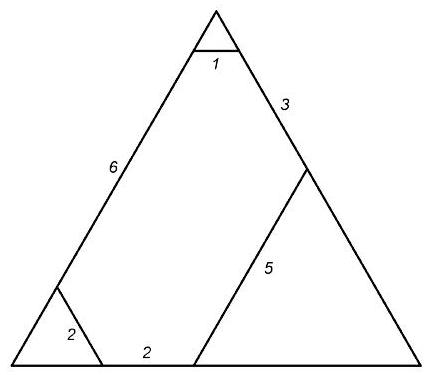
\includegraphics[max width=\textwidth, center]{2024_11_21_f6035da02386d0911452g-1}


\end{document}